\hypertarget{part-2-treemap-1}{%
\section{Part 2, Treemap 1}\label{part-2-treemap-1}}

\begin{figure}

%\caption{Treemap 1}
\end{figure}

\centering
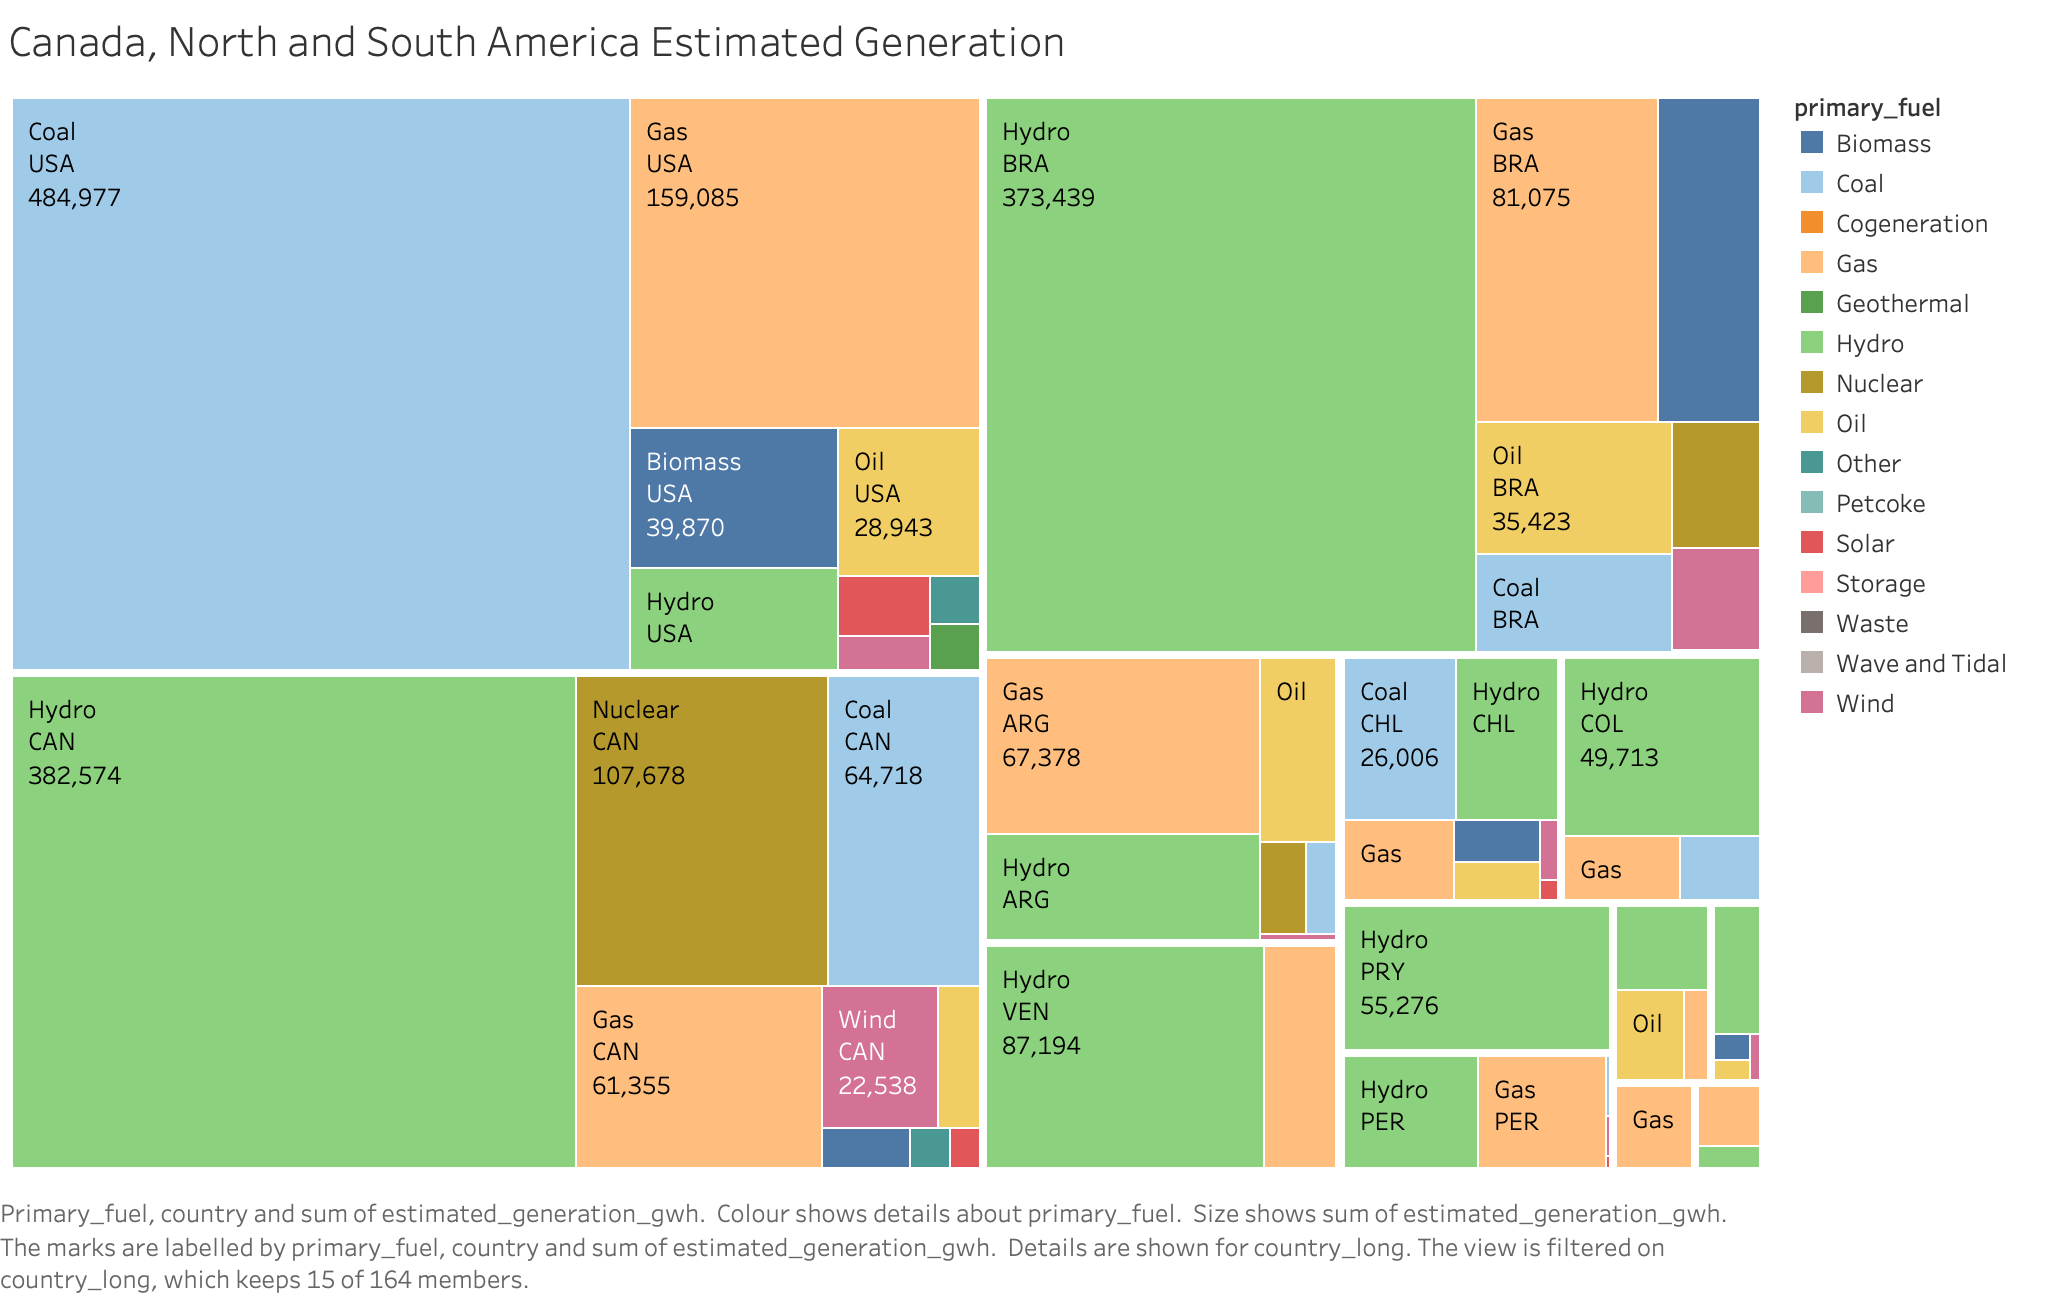
\includegraphics[width=15cm]{AmericaEstGeneration}

\begin{itemize}
\tightlist
\item
  \textbf{Name of Tool}: Tableau
\item
  \textbf{Country}: All of north, central and south america.
\item
  \textbf{Year}: 2018
\item
  \textbf{Data Preparation}: The data was filtered using the built in features of Tableau, just using the Counties that are avaiable within the dataset assosiated to these contenants. 
\item
  \textbf{Color}: The colour coding is assossiated with the primary fuel type.
\item
  \textbf{Hierarchy}: What is the data hierarchy contained in the
  treemap?
\item
  What leaf node size is mapped to? These are mapped to the total estimated values of energy generated by the different primary fuels.
\item
  How are the leaf nodes laid out or positioned? They are laid within the overall node of the country. For example USA.
\item
  What are internal nodes mapped to? These are assigned to the primary fuel of the power plant.
\item
  What is internal node size mapped to? These are mapped to the total estimated values of energy generated by the different primary fuels.
\item
  Which treemap node layout algorithm is used?
  Tableau built in algorithm.
\end{itemize}
